\documentclass{article}
% General document formatting
\usepackage[margin=0.7in]{geometry}
\usepackage[utf8]{inputenc} % UTF characters
\usepackage{amsmath,amssymb,amsfonts,amsthm} % Math stuff
\usepackage{lipsum} % Random text
\usepackage{graphicx} % For figures
\usepackage{float} % Floating figure inside the text

\newcommand{\ten}[1]{\boldsymbol{\mathcal{#1}}}
\newcommand{\mat}[1]{\mathbf{#1}}
\renewcommand{\vec}[1]{\mathbf{#1}}
\newcommand{\R}{\mathbb{R}}

\title{Fast Matrix-Vector Multiplication in Kronecker Form}

\author{Oguz Kaya and Olivier Coulaud}

\date{}

\begin{document}

\maketitle

\section{Background and Motivation}

Tensors, or multi-dimensional arrays, are structures that generalize vectors and matrices to higher dimensions.
Specifically, $\ten{X} \in \R^{N_1 \times N_2 \times \dots \times N_D}$ is an $D$-dimensional tensor with elements $x_{i_1, \dots, i_D} \in \R$ where $1 \le i_d \le N_d$ for all $1 \le d \le D$.
Tensor-based computations have witnessed a remarkable increase in popularity in the last two decades due to great advancements in tensor theory and algorithms as well as their expressive power for high-dimensional algebraic structures that appear in fundamental applications in computational biology, chemistry, physics, signal processing, data analysis, and machine learning.
Tensors are particularly useful when the problem at hand either has or can be reformulated to exhibit a high-dimensional structure.
In this formulation, ``high-dimensional'' matrices and vectors of size $N^D \times N^D$ and of size $N^D$, respectively, are expressed as $2D$- and $D$-dimensional tensors, respectively, of size $N$ in each dimension.
In most cases, the inherent structure and properties of the problem that form these matrices/vectors~(and corresponding tensors) imply a ``low-rank'' property; matrices and vectors can be expressed using polynomial number of elements in $N$ and $D$~(instead of $N^{2D}$ or $N^D$ elements), which is rendered possible via so-called \emph{tensor decompositions}.
Once matrices and vectors are expressed in this form, all matrix and vector operations such as matrix-vector multiplication and basic vector arithmetic~(addition, subtraction, multiplication/division by a scalar, inner product) are performed under this ``compressed'' scheme with tremendous gains in terms of computational and memory costs.

One of the most popular tensor decompositions used in this context is called \textit{tensor-train decomposition}.
A matrix of size $N^D \times N^D$ is expressed via \textit{tensor-train network} of $D$ 4-dimensional tensors of size $N \times N \times R_A \times Q_A$, where ($R_A, Q_A)$ denotes the rank of the matrix in the tensor-train form.
Similarly, a vector $\vec{x}$ of size $N^D$ comprises $D$ 3-dimensional tensors of size $N \times R_x \times Q_x$.
An anologous way to interpret these tensors would be to consider them as matrices~(or vectors) of size $N \times N$~(or $N$), where each element in the matrix~(vector) is a matrix of size $R_A \times Q_A$.
We will be exclusively working on a fundamental kernel involving the multiplication of such \textit{matrix/vector of matrices} described in what follows.

\section{Matrix-vector multiplication in Kronecker form}

Matrix-vector multiplication is a fundamental computational kernel in scientific computing whose optimization plays a key role in obtaining high performance linear and non-linear solvers.
For a given matrix $\mat{A} \in \R^{M \times N}$ and a vector $\vec{x} \in \R^{N}$, the multiplication $\vec{y} = \mat{A} \vec{x}$ is defined as $y_i = \sum_{j = 1}^{N} A_{i, j} x_j$ where $\vec{y} \in \R^{M}$.

Here, we will consider a generalized version of the standard matrix-vector multiplication, involving a \textit{matrix of matrices} and a \textit{vector of matrices}, i.e., $\mat{A}_{i, j}, \mat{x}_j$ and $\mat{y}_i$ are matrices.
In describing this computation, we are in need of a special operation called \textit{Kronecker product} on matrices, which is defined in what follows.

The \emph{Kronecker product} of two matrices $\mat{B} \in \R^{M_B \times N_B}$ and $\mat{C} \in \R^{M_C \times N_C}$ is denoted by the operation $\otimes$ and results in a matrix $\mat{D} = \mat{B} \otimes \mat{C}, \mat{D} \in \R^{M_B M_C \times N_B N_C}$, which is defined as
\begin{equation}
  \mat{D} = \mat{B} \otimes \mat{C} = 
  \begin{pmatrix}
    B_{1,1} \mat{C}    & \cdots & B_{1, N_B} \mat{C}   \\
    \vdots       & \ddots & \vdots         \\
    B_{M_B, 1} \mat{C} & \cdots & B_{M_B, N_B} \mat{C} \\
  \end{pmatrix}
  \label{eq:kron}
\end{equation}

We now define an operation we call \textit{matrix-vector multiplication in Kronecker form~(MxVK)} as follows.
Given a matrix of $M \times N$ matrices $\mat{A}$ such that $\mat{A}_{i, j} \in \R^{R_A \times Q_A}$ for some fixed $R_A, Q_A$ for all $1 \le i, j \le N$, and a vector of $N$ matrices $\vec{x}$ such that $\vec{x}_j \in \R^{R_x \times Q_x}$ for some fixed $R_x, Q_x$ for all $1 \le j \le N$, the result of the MxVK yields a vector $\vec{y} = \mat{A} \vec{x}$ of $M$ matrices with entries 
\begin{equation*}
  \vec{y}_i = \sum_{j = 1}^{N} \mat{A}_{i, j} \otimes \vec{x}_j, \hspace{1em} \vec{y}_i \in \R^{R_A R_x \times Q_A Q_x}
  \label{eq:mxvk}
\end{equation*}
Note that when $R_A = Q_A = R_x = Q_x = 1$, MxVK reduces to standard matrix-vector multiplication as $\mat{A}_{i, j}$,$\vec{x}_j$ and $\vec{y}_i$ become scalars and Kronecker product reduces to scalar multiplication.
We provide a pictorial representation of this operation in the following figure in which the computation of $\vec{y}_2 = \sum_{j = 1}^{N} \mat{A}_{2, j} \otimes \vec{x}_j$ is highlighted.
\begin{figure}[H]
\centering
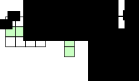
\includegraphics[width=0.5\linewidth]{mxvk.pdf}
\end{figure}

A $D$-dimensional tensor/vector in tensor-train form comprises $D$ matrices/vectors $\mat{A}^{(d)}$/$\vec{x}^{(d)}$, $0 \le d < D$ in this form each potentially having different sizes $M_A^{(d)}, N_A^{(d)}$.
Their ranks, however, are linked such that $Q_A^{(d - 1)} = R_A^{(d)}$.
Moreover, for the first and the last matrices, we always have $R_A^{(0)} = Q_A^{(D - 1)} = 1$.
Therefore, we rather denote these ranks in an array $R_A(0), R_A(1), \dots, R_A(D)$~($R_A(0) = R_A(D) = 1)$, in which case the matrix in the dimension $d$ obtains the ranks $R_A(d)$ and $R_A(d + 1)$, respectively.
Matrix-vector multiplication in this form involves an MxVK in each dimension to obtain $\vec{y}^{(d)} = \mat{A}^{(d)} \vec{x}^{(d)}$~(and there it is your first potential parallelism!).

Carrying out matrix-vector multiplication in tensor-train form is a fundamental kernel in low-rank tensor computations and constitutes one of the most expensive steps in the context of an iterative solver.
The goal in this task is to implement very efficient matrix-vector multiplication kernels and effectively parallelize them with different paradigms using OpenMP.

You are already given a skeleton code \texttt{ttmatvec.cpp} that loads a matrix and a vector in tensor train form~(\texttt{TTMat} and \texttt{TTVec}), multiplies them, then writes the results back into another file.
It involves reference non-optimized sequential implementation provided in \texttt{ttvec.h/.cpp} and \texttt{ttmat.h/.cpp}.
You will be implementing your own \texttt{ttvec.h/.cpp} and \texttt{ttmat.h/.cpp} that provides \texttt{TTMat} and \texttt{TTVec} structures/classes with all functions whose signatures are provided in \texttt{ttmatvec.cpp} so that we can replace the reference implementation with your code to test its performance.

In order to create \texttt{TTMat}s and \texttt{TTVec}s, we provide two executables \texttt{create-ttmat} and \texttt{create-ttvec} that generate random structures of specified sizes in a binary file.
Run these executables without parameters to see their usage.
Note that in these executables, to create a $D$ dimensional TTMat/TTVec, we pass $D - 1$ ranks as the rank in the first and the last dimension are always $1$.

The first entry in the binary file for a \texttt{TTMat} is an integer representing $D$.
This is followed by $D$ integers representing the number of rows of matrices in each dimension (i.e. $M_A^{(d)}$).
The next $D$ integers provide the number of columns of matrices in each dimension~(i.e., $N_A^{(d)}$.
Afterwards, there are $D - 1$ integers containing the ranks $R_A(1), \dots, R_A(D - 1)$~($R_A(0)$ and $R_A(D)$ are always $1$ hence not given in the file).
In the rest of the file, we have \texttt{double} elements representing the matrices in dimensions $0, \dots, D - 1$, respectively.
The matrix for the dimension $d$ contains $M_A^{(d)} \times N_A^{(d)} \times R_A{(d)} \times R_A{(d + 1)}$ \texttt{double} entries.
Each matrix of size $M_A^{(d)} \times N_A^{(d)}$ in dimension $d$ is stored in column-major layout, and each block of size $R_A^{(d)} \times R_A^{(d + 1)}$ within this matrix is also stored in column-major layout.
\texttt{TTVec} binary file is defined similarly, except that there is no $N_A^{(d)}$.
Have a look at the load/save/print routines in \texttt{ttmat.cpp} and \texttt{ttvec.cpp} if you have any doubts about the data orientation.
In your implementation, you should provide an input/output interface~(with functions \texttt{loadTTMat}/\texttt{loadTTVec}/\texttt{saveTTVec} that can read/write a TT structure in a binary file.
In your internal data structures for the matrix-vector multiplication algorithm, you are free to change the data orientation and storage as you will, but the resulting vector that you write to output must follow this column-major layout so that we can compare the results.
Setup your internal data structures in \texttt{loadTTMat} and \texttt{loadTTVec}.
These two function calls will not be timed for performance, so you can fine-tune your layout here without worrying about timing.
Any computation in these functions pertaining to actual matrix-vector multiplication will be considered cheating, however!

Once your implementation writes the resulting vector $\vec{y}$ in a binary file, you can compare your results with the results of the reference implementation using \texttt{compare-ttvec} executable.
Make sure your implementation is CORRECT before being OPTIMIZED, as you will get 0 score for a test case if the result is incorrect.

Do not hesitate to take your time to read the provided code and have a look at matrix/vector data structures.
It is always insightful to read the reference implementation and understand how it works, before proceeding to your own implementation.
You will see in the code that MxVK function utilizes another subroutine to perform the Kronecker product of two matrices as in \eqref{eq:kron}, then performs the MxVK using this subroutine as in \eqref{eq:mxvk}.

\section{Tasks}

\subsection{Optimizing sequential MxVK}
In this first task, your goal is to optimize the given MxVK kernel as much as possible.
Take particularly into consideration the fact that matrices $\mat{A}_{i, j}$ and $\vec{X}_{j}$ are relatively small~(e.g. $\le 128$ in each dimension).
A good start would be determining the total number of flops performed in MxVK, the total amount of data ``touched'' during this computation~(or total mops~(memory operations)) in terms of $N$, $R_A$ , and $R_x$.
Finally, $\#flops / \#mops$ gives the computational intensity of this operation, which you should aim to attain with an optimized implementation.
Once you are able to attain the computational intensity, do not hesitate to employ vectorization using AVX to crunch all this intensity if possible.

Explain each optimization technique you employed, and report the time difference with respect to previous baseline.
Also report how well your code performs with respect to different set of parameters~(i.e., small or large $M_A, N_A, R_A, Q_A, M_x, R_x, Q_x$), and try to fine-tune your code for edge cases if possible.

You are \textbf{NOT} allowed to use any sort of parallelization for this task. You are indeed allowed, however, to employ this optimized kernel in the following tasks requiring parallelization.

\subsection{Parallelization using OpenMP}
Now that you have a working sequential implementation, it is time to optimize it to the fullest and obtain the best performance.
Here, you will parallelize the optimized sequential implementation you provided in the prevoius case using OpenMP parallel constructs.
You are free to use parallel loops or sections.
You are also welcome to make significant changes to your sequential implementation, in which case you would need to report why you needed such a change from a performance point of view.
Make sure your paralellization scales acceptably well for pathological input sizes as well (i.e., $N_A$ very small, $R_A$ small, $R_x$ large, etc.).
Explain your parallelization strategy, how you divide the work among threads, achieve load balance, handle data dependencies, perform synchronization~(if necessary), etc.
Think about optimizing your parallelization on a single as well as multiple NUMA sockets as we will test the performance using multiple sockets as well.
To restrain your code to work on a single socket, use the command $numactl -N 0 ./ttmatvec .....$.

\subsection{Parallelization using OpenMP tasks}
You are \textbf{NOT} allowed to have any other means of parallelization for this assignment except OpenMP tasks.

You will now do another parallel implementation, but this time using OpenMP tasks.
Note that your implementation should \textbf{NOT} be a simple re-wrapping of your previous parallelization with loops; you should try to extract finer-grain parallel tasks that have elegant output independence hence can be executed in parallel efficiently, but are coarse enough that it would not kill the performance due to tasking overhead.
The performance will be similarly tested on a single and multiple NUMA sockets.

\section{General guidelines and considerations}

\begin{itemize}

\item You can assume that $1 \le R_A, R_x \le 128$, and $1 \le N \le 1024$.

\item It might be useful to take into consideration the machine parameters~(particularly the cache size at different levels, which you can query using \texttt{lscpu} command on Linux).

\item Grading will be based on the speed of execution of your kernels.
We will run each kernel multiple times and take the median.
You should also be writing a report summarizing your approaches for optimization, and performance gains you obtained from each approach.

\item The quality of your code~(documentation, indentation, using proper functions, etc.) will also have an impact on your final score~(i.e. we will subtract some points depending on how ugly the code is .) ).

\item Since we focus on parallelization, you are also encouraged to parallelize the work among the group members.
For instance, sequential optimization and parallelization could be done in parallel!
And task-based parallelization and OpenMP parallelization are independent as well!.

\end{itemize}

\end{document}
